\documentclass{article}

\usepackage{amsmath} 
\usepackage{subfigure}
\usepackage{caption}
\usepackage{listings}
\usepackage[twocolumn,textwidth=17.31cm,columnsep=.81cm]{geometry}

\usepackage{graphicx}
\usepackage{breqn}

\lstset{ %
 basicstyle=\small,
 breaklines=true,
 }

\begin{document}
\title{Solving Captchas with an OCR system}
\author{Sebastian Agethen, D01944015 \\ Lin Sheng-Ching, R99222030 \\ Jeroen Dhondt, A01922201 }

\onecolumn

\maketitle

\tableofcontents

\twocolumn

\section{Introduction}
\section{Implementation}
We first introduce the structure of our system. In the following sections we then present each step in greater detail.

\subsection{General structure}
Our OCR system runs in two stages, a training phase and a live phase. In the training phase, each our our features is evaluated on a set of 36 Bitmaps describing the characters we can recognize. Currently, this encompasses the 26 capital characters of the English alphabet as well as the digits 0 to 9. In the second phase, called live phase, we extract segments from an input file and then compute all features for each segment. Finally, training data and live data are passed together with a weight vector to a clustering method, which finds either the closest or the k-closest matching results.

\subsection{Preprocessing}

\subsubsection{Quantization}
For our quantization, we first set a threshold value t, and then evaluate the Eq.~\ref{eq:threshold}. If the term $v < t$, then we set the pixel $p = 0$, otherwise if $v \geq t$, we set the pixel $p = 1$.
\begin{equation}
v = \sqrt{r^2 + g^2 + b^2}
\label{eq:threshold}
\end{equation}

\begin{figure}
\subfigure[Original B]{
\includegraphics[width=0.5\textwidth]{images/B.pdf}
}
\subfigure[Quantised B]{
\includegraphics[width=0.5\textwidth]{images/quantised_B.pdf}
}
\caption{Original B v.s. Quantised B}
\end{figure}

\subsubsection{Skeletonization}
After the image is quantized, we repeatedly use the conditional mark pattern and unconditional mark pattern until the nothing is changed. Finally, we use the bridge operation to recover the connectivity of the character. Conditional and unconditional mark patterns for Skeletonization can be found in Fig.~\ref{fig:markpatterns1} to \ref{fig:markpatterns3}, while those for the Bridge operation can be found in Fig.~\ref{fig:bridge}.

The comparison of the skeletonization can be seen in the Fig.~\ref{fig:skeleton}.
\begin{figure}
\subfigure[Quantised B]{
\includegraphics[width=0.5\textwidth]{images/quantised_B.pdf}
}
\subfigure[Skeletonized B]{
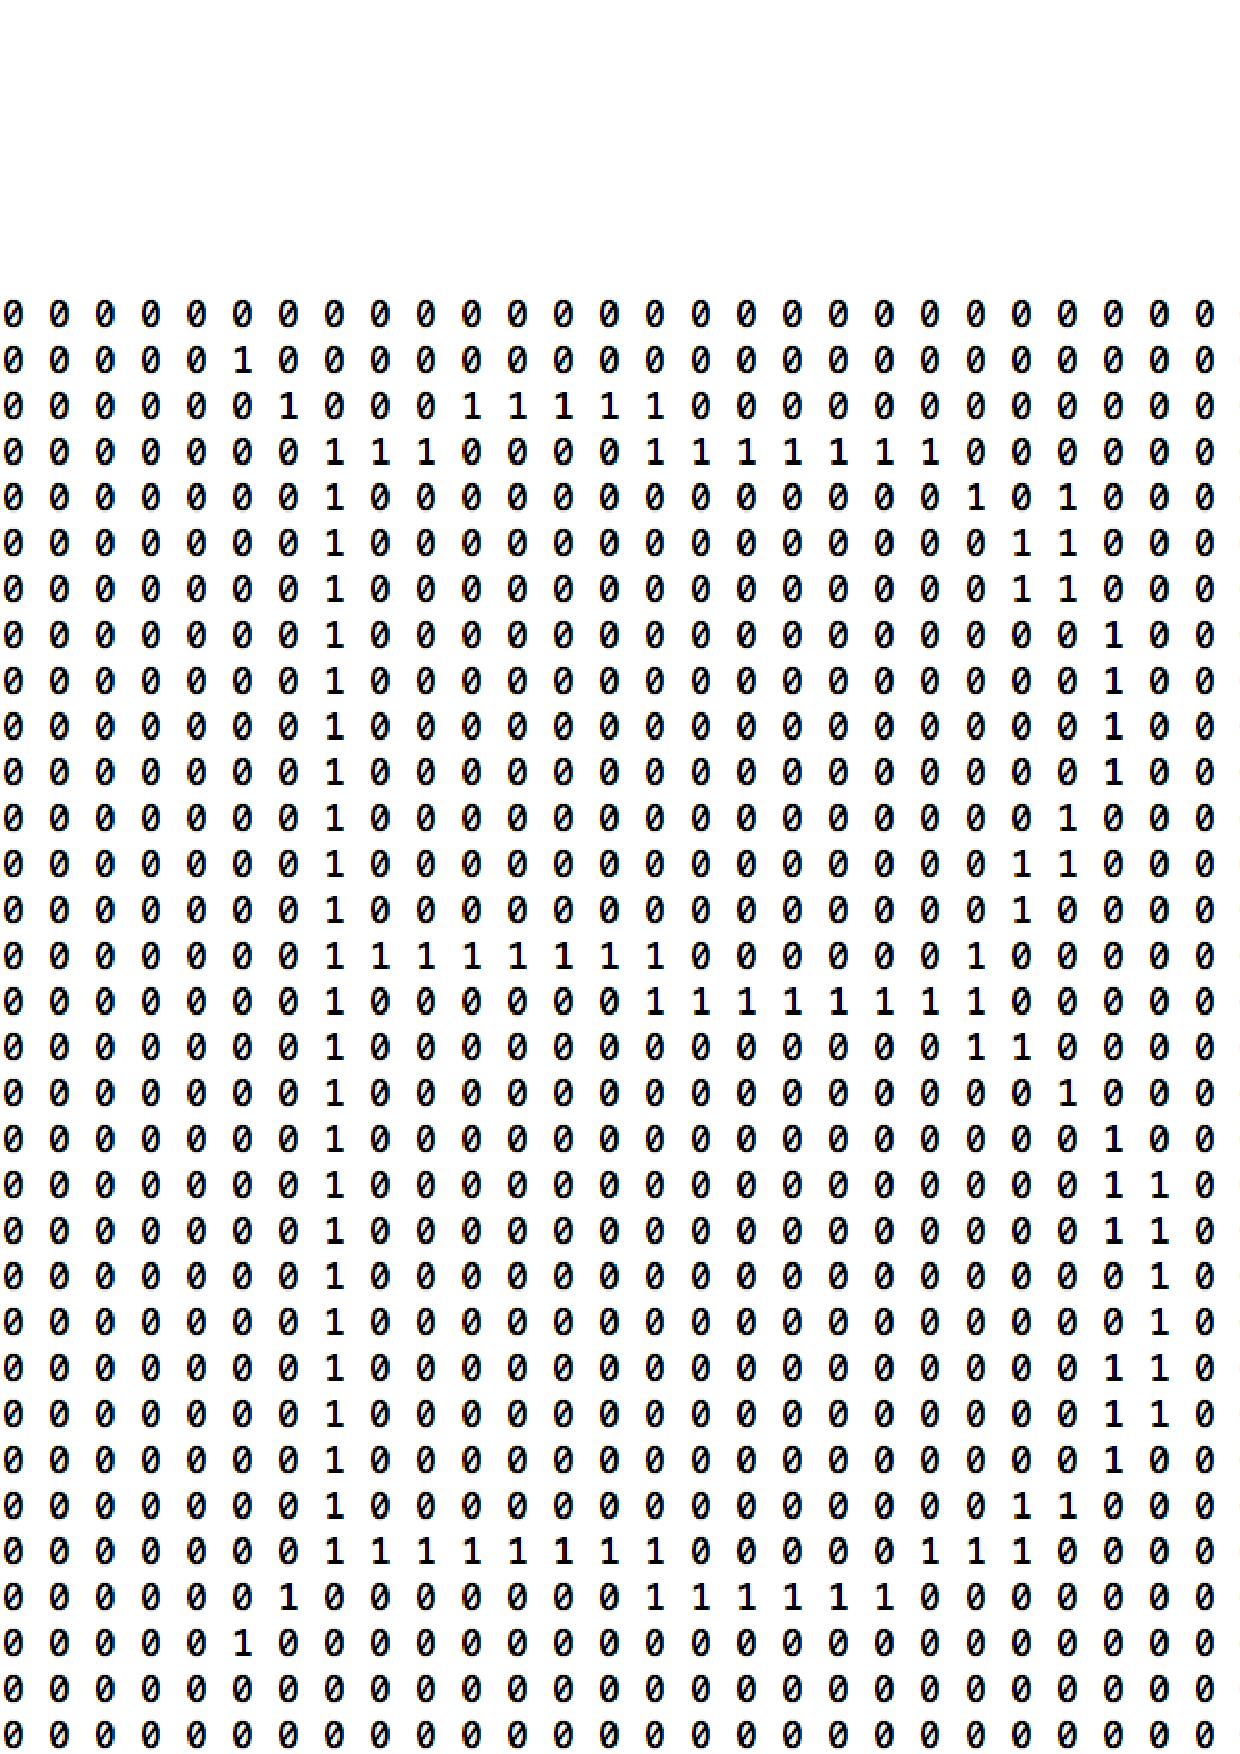
\includegraphics[width=0.5\textwidth]{images/skeletonized_B.pdf}
}
\caption{Qunatized B v.s. Skeletonized B}\label{fig:skeleton}
\end{figure}

\subsubsection{Boundary extraction}
The algorithm to extract the boundary of character can be seen in the listing~\ref{lst:boundary}.
\begin{lstlisting}[caption={Boundary Extraction algorithm},label={lst:boundary}]
1. Scan the pixel from left to right for each row.
2. When the gradient changes strictly, set the row number as the ceiling of the sentence.
3. After finding the ceiling, keep scanning the pixels. If we find a totally white row, set the row number - 1 as the bottom of the sentence.
4. Scan the pixels of each column from the ceiling to the bottom.
5. When the gradient changes strictly, set the column number as the left boundary of the sentence.
6. After finding the left boundary, scan the pixels from the rightmost pixel to the left, from ceiling to the bottom. As we find a strict gradient of the column, set it as the right boundary.
7. Keep doing the steps 1 ~ 6 until all the input file is scanned.
8. For each sentence, set the left boundary as the left boundary of the first chacter and scan the pixel from ceiling to the bottom, starting from the left.
9. If there is a column totally white, set the column number -1 as the right boundary of the chacter.
10. Keep scanning until a strict gradient occurs. Set the column number as the left boundary of the next chacter.
11. Keep scanning until another strict gradient column is found and the right boundary of the chacter is set.
12. Repeat step 9 ~ 11 until the sentence is totally scanned and scan the next sentence.
\end{lstlisting}

\subsubsection{Orientation}

The followings are the derivation of the orientation angle of an object:
Define the (m,n)th spatial moments
\begin{multline}
M(m,n)=\frac{1}{J^n K^m}\sum_{j=1}^J\sum_{k=1}^K (x_k)^m (y_j)^n F(j,k)
\end{multline}
where $x_k=k-\frac{1}{2}, y_j=J+\frac{1}{2}-j$ and
\begin{multline}
U(m,n)= \\ \frac{1}{J^n K^m}\sum_{j=1}^J\sum_{k=1}^K \left(x_k-\frac{M(1,0)}{M(0,0)}\right)^m  \left(y_j-\frac{M(0,1)}{M(0,0)}\right)^n F(j,k)
\end{multline}
where $x_k=k-\frac{1}{2}, y_j=J+\frac{1}{2}-j$ and then find the maximum value of eigen value

\begin{align}
&E^T U E = \Lambda\\
&E=\begin{bmatrix}
 e_{11}&e_{12} \\ 
 e_{21}&e_{22} 
\end{bmatrix}
\\
&\Lambda=\begin{bmatrix}
 \lambda_1&0 \\ 
0 & \lambda_2
\end{bmatrix}
\end{align}
By calculation, 
\begin{multline}
\lambda_1=\frac{1}{2}\left[U(2,0)+U(0,2)\right] + \\ \frac{1}{2}\left[U(2,0)^2+U(0,2)^2-2U(2,0)U(0,2)+4U(1,1)^2\right]^{1/2}
\end{multline}
\begin{multline}
\lambda_2=\frac{1}{2}\left[U(2,0)+U(0,2)\right] - \\ \frac{1}{2}\left[U(2,0)^2+U(0,2)^2-2U(2,0)U(0,2)+4U(1,1)^2\right]^{1/2} 
\end{multline}
\begin{multline}
\rightarrow \theta=\arctan{\left[ \frac{\lambda_M - U(0,2)}{U(1,1)} \right] }
\end{multline}

\subsubsection{Convex Hull}
\label{sec:convexhull}

We define the \textit{Convex Hull} of a character as follows: Given that the input is already quantized to black-and-white, where white is the background, any point that is on a line between any two black points has to be black, too. More formally, this can be expressed as:

\begin{align}
&\forall v_1, \forall v_2 \in \text{B}: v_t \in \text{C},
&v_t = (1-t)v_1 + t v_2, t \in [0,1]
\end{align}
where $B$ is the set of black pixels and $C$ is the Convex Hull. An example can be found in Figure \ref{fig:convex} for the character 'X'.

\begin{figure}
 \centering
  \subfigure[]{
  \includegraphics{images/X.png}
 }
 \subfigure[]{
  \includegraphics{images/X_convex.png}
 }
\caption{Convex Hull for the character 'X'. a) Original character, b) Convex Hull of character}
\label{fig:convex}
\end{figure}

\subsection{Features}
In the following we present each feature we used in detail.

\subsubsection{Geometrical features}
\label{sec:geometrical}
%Area, weight center, diameter, etc
Our geometical features consist of area, weight center, average and maximum distance from weight center.
\paragraph{Area}
Calculate the total number of pixels

\paragraph{Weight center}
\begin{equation}
F_c=\frac{\sum F(i,j)x_{i,j}}{\sum x_{i,j}}
\end{equation}

\paragraph{Average distance from weight center}
\begin{equation}
d = \sqrt{\frac{\sum_{i,j}(x_{i,j} - F_c)}{\sum_{i,j}x_{i,j}}}
\end{equation}

\paragraph{Maximum distance from weight center}
\begin{equation}
	d_M = MAX(\sqrt{x_{i,j}-F_c})
\end{equation}

\subsubsection{Bays, Lakes and the Euler number}
\label{sec:lakeseuler}
Each character posseses a property called the \textit{Euler number}, which we define as the number of \textit{Connected Components} minus the number of \textit{Lakes}.

In a bitmap that consists of only two colors (e.g., black-and-white), we define a \textit{Lake} to be a connected area which does not reach the borders of the \textit{Convex Hull} (see Section \ref{sec:convexhull}) and is colored with the background color (e.g., white). A related term, the \textit{Bay} is defined to be a connected area of background color that does touch the borders of the \textit{Convex Hull}. The last term is that of a \textit{Connected Component}. For our purposes it will describe any connected area of non-background color (e.g., black). An example for each term is given in Figures \ref{fig:bayslakescomp} a) to d) with the capital character 'A' .

\begin{figure}
 \centering
 \begin{subfigure}[]
  \centering
  \includegraphics[height=2cm]{images/A_original.png}
  \label{fig:original}
 \end{subfigure}
%
 \begin{subfigure}[]
  \centering
  \includegraphics[height=2cm]{images/A_bay.png}
  \label{fig:bays}
 \end{subfigure}

 \begin{subfigure}[]
  \centering
  \includegraphics[height=2cm]{images/A_lake.png}
  \label{fig:lakes}
 \end{subfigure}
%
 \begin{subfigure}[]
  \centering
  \includegraphics[height=2cm]{images/A_component.png}
  \label{fig:ccomp}
 \end{subfigure}
 \caption{a) Original character, b) 'A' has a single bay (colored red), c) 'A' has one lake, d) 'A' has one Connected Component. Thereby 'A' has Euler number 0 }
 \label{fig:bayslakescomp}
\end{figure}

We compute these features in the following fashion: We sequentially scan the given image for white (Bays and Lakes) or black (Connected Components) pixels. Once such a pixel is found, we then execute a coloring algorithm that recursively visits neighbors of the same color and then colors each visited pixel in a third color (e.g., a greytone). If the coloring algorithm is run on a white pixel, we also determine whether we reached the border of the bitmap during execution by setting a flag \texttt{reachedBorder}. Furthermore, after each instance we increase a counter variable for the corresponding type, e.g., \texttt{numberOfLakes}.

This algorithm visits each pixel at most twice, since the coloring algorithm only visits pixels that have not been colored yet, and therefore requires linear time $O(n)$.

\subsubsection{Line and Circle Components}
Another important property of lating characters are the number of straight lines and the number of circles within a \textit{Connected Component}. For an example, please refer to Figure \ref{fig:lines}: The character 'A' is 0 vertical lines, 1 horizontal line and 0 circles. Note that we currently do not count diagonal lines. However, we reserve this feature for our Future Work.

\begin{figure}
 \centering
 \subfigure[]{
  \includegraphics[height=2cm]{images/A_skel_line.png}
 }
 \subfigure[]{
  \includegraphics[height=2cm]{images/A_boundary.png}
 }
 
 \caption{a) In Red: Skeleton of 'A' having one horizontal line, b) Boundary Extraction: Two horizontal lines}
\label{fig:lines}
\end{figure}

We use a very simple method to count straight lines: We first search a pixel that is not of background color. Once it is found, we then visit the next pixel in one direction recursively and thereby determine the length of a possible line. For example, to compute horizontal lines and given that the current pixel is located at (x,y), we visit (x+1,y), (x+2,y) and so on until a different color is encountered. We then count the line if its length meets a predetermined threshold.

A major issue with this algorithm arises when lines have a thickness of more than one pixel: In that case, for varying sizes of characters, varying number of lines would be found! It is therefore imperative to first do preprocessing. We suggest to use either \textit{Skeletonization} or \textit{Boundary Extraction}. When using \textit{Skeletonization}, each line of a character is shrunk to a thickness of 1, enabling easy parsing. When using \textit{Boundary Extraction} however, two lines are (usually) created. In our implementation, we have used \textit{Boundary extraction}.

We can also count the number of circles in a character. To do this, we find a \textit{Lake} (see Sec.~\ref{sec:lakeseuler}) and determine the following formula:
\begin{equation}
C_0 = \frac{4\pi A_0}{P_0^2}
\end{equation}

where $A$ is the area of the Lake and $P$ is the \textit{Perimeter}, i.e., the number of neighboring pixels.

\subsubsection{Shape Context}
We include a method proposed by Belongie et al. \cite{Belongie00shapecontext:} as a feature: Shape Descriptors. A Shape Descriptor is a single value that describes how similar two shapes are, where a value is 0 when two shapes are identical, and $>0$ otherwise. 

\begin{figure}
 \centering
 \includegraphics[width=8cm]{images/samples.png}
 \caption{Sampling process: Left: Perform Boundary Extraction, Center: Choose a fixed number of random samples, Right: Compute log-distances between samples}
\end{figure}

The authors construct this value by sampling a picture, computing the distances between samples and then creating a histogram for each sample. When comparing two shapes, the Chi-Square distance 

\begin{displaymath}
C_S = \frac{1}{2} \sum\limits^K_{k=1} \frac{\left[g(k) - h(k)\right]^2}{g(k)+h(k)}
\end{displaymath}


is computed for each pair of histograms of shape A (g in the formula above) with histograms of shape B (h). This would result in $n^2$ values! The suggested solution is to find a bipartite matching between samples of shape A and B and then compute the sum of all matched chi-square distances.

\subsection{Decision mechanism}
Once every feature has been evaluated on all segments, we need to decide which character a segment resembles. In our system, we use a simple clustering algorithm.

\subsubsection{Weight vector}
An important point to notice is that above features are not normalized. The \textit{Euler number} of a character may range between -1 and 1, while the total black area of a segment may easily have ~300 pixels for letter of font size 32. Normalizing all values would improve results greatly. However, another problem occurs: In reality, the Euler number distinguishes a character far more than the area. We would like to \textbf{weigh} the Euler number higher than the area. To achieve this, we must therefore include a weight-vector. 

\subsubsection{Clustering}

Once this is done, the clustering algorithm is very straightforward: For each segment a vector is created, where each dimension of the vector resembles another feature. Each component of a vector is furthermore multiplied by the corresponding entry in the weight-vector. 

We then choose the vectors found in our training phase to be the cluster centroids. For all other vectors, namely those found in the live phase, we compute the distances to all cluster centroids and then assign it to the closest centroid. The advantage of this method over, e.g., a decision tree is that we can also support k-next-neighbor request, which is useful for post-processing. As we currently do not do any post-processing, we keep this matter for our Future Work.

\section{Experimental Results}

We evaluate our program on the text seen in Figure \ref{fig:input}. The text contain Capitals form the English alphabet as well as the digits 0 to 9.
%\begin{lstlisting}[caption={Input for our evaluation},label={lst:input}]
%ABCDEFGHIJKLMNOPQRSTUVWXYZ0123456789
%AN APPLE A DAY KEEPS THE DOCTOR AWAY
%\end{lstlisting}

\begin{figure}[ht]
 \includegraphics[width=8cm]{images/demo.png}
 \caption{Input Bitmap for our evaluation}
 \label{fig:input}
\end{figure}

\newpage

\begin{lstlisting}[caption={Result of our evaluation},label={lst:output}]
Detected: 
ABZDEFDHG2SLNNORORETKXQWYZD5ZB4ZB5BB
Diff:
  C   G IJK M  PQ S UVWX  0123 56789
(22 Errors)

Detected:
ANARRLEADAYSEERETHEDOZTORAQAY
Diff:
   PP      K  PS     C    W  
(7 Errors)
\end{lstlisting}

The output of our OCR system can be seen in Listing \ref{lst:output}. From the total of 65 characters, we did not correctly recognize 29, giving an overall error-ratio of 44.6\%.
We notice that with our current features, the recognition is far better for alphabetical characters than for numbers. From ten digits only one was correctly identified (Error ratio: 90\%), while of the 55 alphabetical characters 35 were correctly identified (Error ratio: 36.3\%). 

\subsection{Discussion}
We now discuss the known flaws of our system leading to the low recognition rate seen above. First of all, some of the features are not well implemented resulting in incorrect values, e.g., our Number of Bays feature. The problem here is that during the computation of the Convex Hull some pixels are falsely included. These pixels then form small Bays that distort our results.

Another problem we met can be revealed from closer study of Fig.~\ref{fig:input}: Notice that the spacing between each character is quite wide. If this is not the case, it may happen that two characters are joined during segmentation. One problem is that characters may overlap, another one is the quantization. Characters in the bitmap are not necessarily black-and-white, but diffuse. It is therefore important to find a good Quantization threshold: Is the threshold too high, characters maybe joined due to diffusion. Is the threshold too low, some characters might be split up, especially for small font sizes.

Finally, we also note that adjusting the weights is critically important for a good result. This issue is a keypoint for any Future Work on this project.

\section{Conclusion}

\section{Division of Labor}

\begin{tabular}{|l|l|}
 \hline
 Sebastian Agethen & Program Framework, Decision Clustering, \\
  & Features: Lakes, Euler number, \\
 & Lines and Circles, Shape Coefficient\\
\hline
 Lin Sheng-Ching & Extraction of characters, \\
 &  skeletonization of characters\\
  & geometrical features (Sec.~\ref{sec:geometrical}), \\ & orientation \\
\hline
 Jeroen Dhondt & Project Proposal, Bays, \\
 & Presentation/Final Report: Introduction, \\
 & Motivation, Conclusion\\
\hline
\end{tabular}


\begin{figure*}
 \includegraphics{images/bridge.pdf}
 \caption{Conditions for Bridging a Pixel, taken from \cite{Pratt:2001:DIP:516234}, p. 406}
 \label{fig:bridge}
\end{figure*}

\begin{figure*}
 \includegraphics[page=1,height=19cm]{images/patternTables.pdf}
 \caption{Unconditional and Conditional Mark Patterns (part 1), taken from \cite{Pratt:2001:DIP:516234}, p. 413}
 \label{fig:markpatterns1}
\end{figure*}

\begin{figure*}
 \includegraphics[page=2,height=19cm]{images/patternTables.pdf}
 \caption{Unconditional and Conditional Mark Patterns (part 2), taken from \cite{Pratt:2001:DIP:516234}, p. 414}
 \label{fig:markpatterns2}
\end{figure*}

\begin{figure*}
 \includegraphics[page=3,height=19cm]{images/patternTables.pdf}
 \caption{Unconditional and Conditional Mark Patterns (part 3), taken from \cite{Pratt:2001:DIP:516234}, p. 415}
 \label{fig:markpatterns3}
\end{figure*}


\bibliography{report}
\bibliographystyle{plain}
\end{document}
